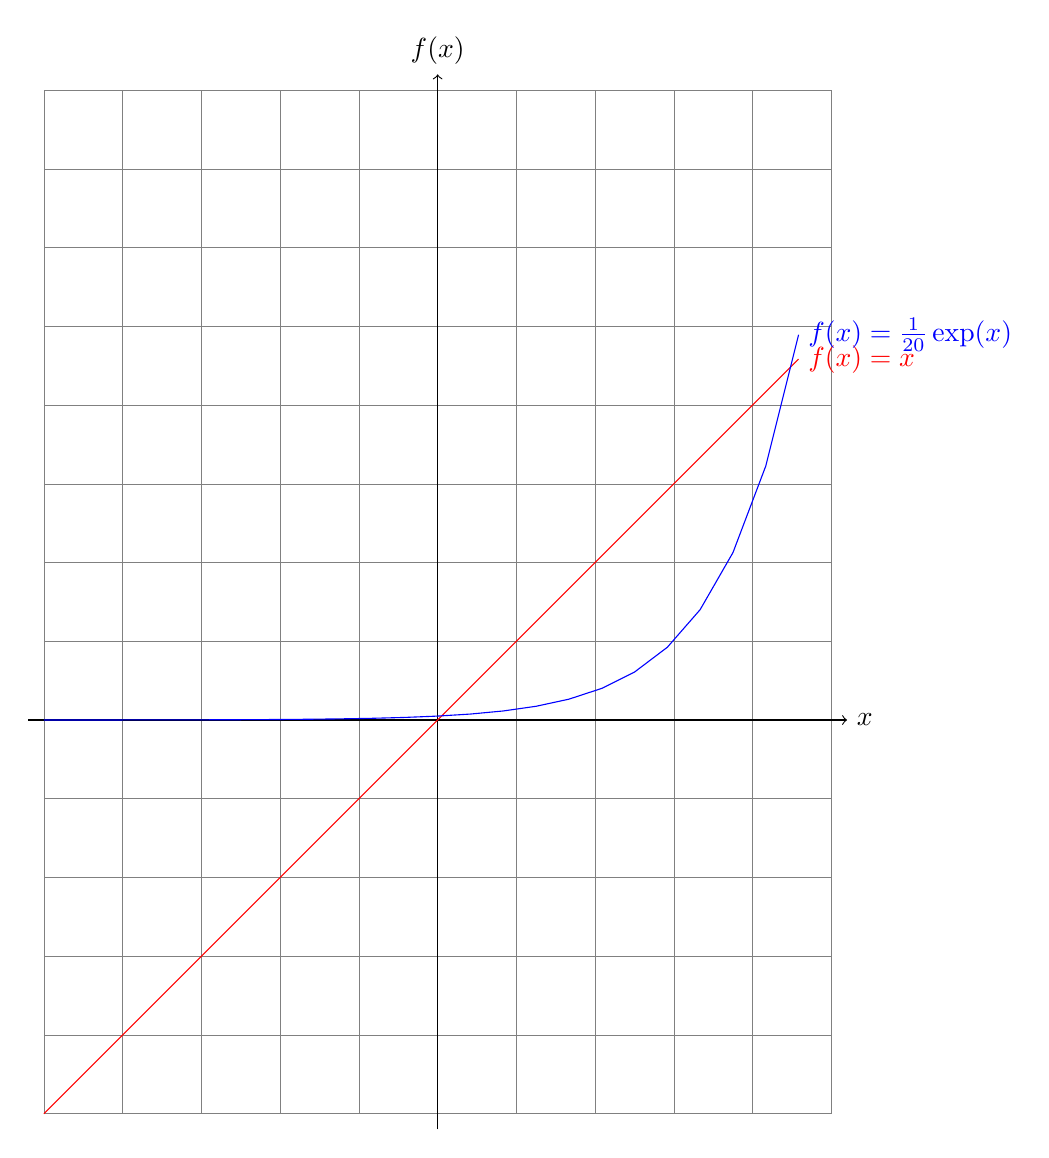
\begin{tikzpicture}
  \draw[very thin,color=gray] (-5,-5) grid (5,8);
  \draw[->] (-5.2,0) -- (5.2,0) node[right] {$x$}; 
  \draw[->] (0,-5.2) -- (0,8.2) node[above] {$f(x)$};
  \draw[color=red]    
    plot (\x,\x) node[right] {$f(x)=x$}; 
  \draw[color=blue] 
    plot (\x,{0.05*exp(\x)}) node[right] {$f(x) = \frac{1}{20}\exp(x)$};
\end{tikzpicture}